\documentclass{scrartcl}
        \usepackage{xcolor, tikz}
        \usepackage{pgfplots}
        \pgfplotsset{compat=newest}
        \pagestyle{empty}
        \definecolor{pdg2112}{RGB}{228,26,28}
\definecolor{pdg2212}{RGB}{55,126,184}
\definecolor{pdg1000010020}{RGB}{153,153,153}
\definecolor{pdg1000020040}{RGB}{166,86,40}
\definecolor{pdg11}{RGB}{152,78,163}
\definecolor{pdg22}{RGB}{77,175,74}
\begin{document}
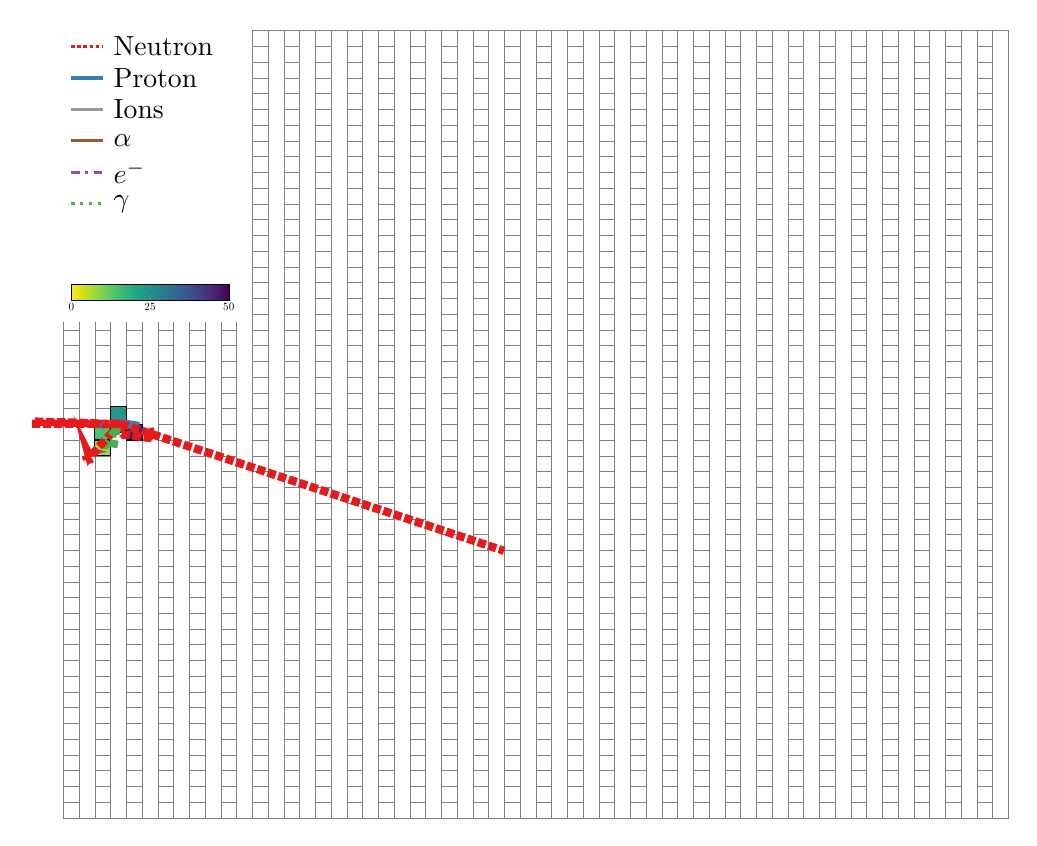
\begin{tikzpicture}[scale=0.4] %\columnwidth/252.0pt]
\draw[step=0.5,very thin,gray] (-0.001000,-12.499) grid (0.500000,3.25);
\draw[step=0.5,very thin,gray] (0.999000,-12.499) grid (1.500000,3.25);
\draw[step=0.5,very thin,gray] (1.999000,-12.499) grid (2.500000,3.25);
\draw[step=0.5,very thin,gray] (2.999000,-12.499) grid (3.500000,3.25);
\draw[step=0.5,very thin,gray] (3.999000,-12.499) grid (4.500000,3.25);
\draw[step=0.5,very thin,gray] (4.999000,-12.499) grid (5.500000,3.25);
\draw[step=0.5,very thin,gray] (5.999000,-12.499) grid (6.500000,12.499);
\draw[step=0.5,very thin,gray] (6.999000,-12.499) grid (7.500000,12.499);
\draw[step=0.5,very thin,gray] (7.999000,-12.499) grid (8.500000,12.499);
\draw[step=0.5,very thin,gray] (8.999000,-12.499) grid (9.500000,12.499);
\draw[step=0.5,very thin,gray] (9.999000,-12.499) grid (10.500000,12.499);
\draw[step=0.5,very thin,gray] (10.999000,-12.499) grid (11.500000,12.499);
\draw[step=0.5,very thin,gray] (11.999000,-12.499) grid (12.500000,12.499);
\draw[step=0.5,very thin,gray] (12.999000,-12.499) grid (13.500000,12.499);
\draw[step=0.5,very thin,gray] (13.999000,-12.499) grid (14.500000,12.499);
\draw[step=0.5,very thin,gray] (14.999000,-12.499) grid (15.500000,12.499);
\draw[step=0.5,very thin,gray] (15.999000,-12.499) grid (16.500000,12.499);
\draw[step=0.5,very thin,gray] (16.999000,-12.499) grid (17.500000,12.499);
\draw[step=0.5,very thin,gray] (17.999000,-12.499) grid (18.500000,12.499);
\draw[step=0.5,very thin,gray] (18.999000,-12.499) grid (19.500000,12.499);
\draw[step=0.5,very thin,gray] (19.999000,-12.499) grid (20.500000,12.499);
\draw[step=0.5,very thin,gray] (20.999000,-12.499) grid (21.500000,12.499);
\draw[step=0.5,very thin,gray] (21.999000,-12.499) grid (22.500000,12.499);
\draw[step=0.5,very thin,gray] (22.999000,-12.499) grid (23.500000,12.499);
\draw[step=0.5,very thin,gray] (23.999000,-12.499) grid (24.500000,12.499);
\draw[step=0.5,very thin,gray] (24.999000,-12.499) grid (25.500000,12.499);
\draw[step=0.5,very thin,gray] (25.999000,-12.499) grid (26.500000,12.499);
\draw[step=0.5,very thin,gray] (26.999000,-12.499) grid (27.500000,12.499);
\draw[step=0.5,very thin,gray] (27.999000,-12.499) grid (28.500000,12.499);
\draw[step=0.5,very thin,gray] (28.999000,-12.499) grid (29.500000,12.499);
\draw[very thin,gray] (0,-12.5) -- (30,-12.5) -- (30,12.5) -- (6,12.5);
\definecolor{tempcolor}{rgb}{0.626579,0.854645,0.223353}\draw[fill=tempcolor,fill opacity=1] (1.000000,-1.000000) rectangle (1.500000,-0.500000);
\definecolor{tempcolor}{rgb}{0.296479,0.761561,0.424223}\draw[fill=tempcolor,fill opacity=1] (1.000000,-0.500000) rectangle (1.500000,0.000000);
\definecolor{tempcolor}{rgb}{0.267004,0.004874,0.329415}\draw[fill=tempcolor,fill opacity=1] (1.500000,-0.264413) rectangle (2.000000,0.235587);
\definecolor{tempcolor}{rgb}{0.120565,0.596422,0.543611}\draw[fill=tempcolor,fill opacity=1] (1.500000,0.072254) rectangle (2.000000,0.572254);
\definecolor{tempcolor}{rgb}{0.283072,0.130895,0.449241}\draw[fill=tempcolor,fill opacity=1] (2.000000,-0.500000) rectangle (2.500000,0.000000);
\draw[color=pdg2112, line width=3pt, densely dotted] (-1.0030938642446927, 0.017501063462610694) -- (-0.00311462843424124, 0.01761852026437318) -- (0.48999999999998634, 0.017676441134211286) -- (0.9899999999999863, 0.0177351707545655) -- (1.4899999999999864, 0.017793900374919715) -- (1.8153518598047413, 0.017832115957335453);
\draw[color=pdg1000020040, line width=3pt, solid] (1.8153518598047413, 0.017832115957335453);
\draw[color=pdg1000010020, line width=3pt, solid] (1.8153518598047413, 0.017832115957335453) -- (1.8279555908984093, 0.039438437451325956) -- (1.84062990635814, 0.06052635885262714) -- (1.8491298322770717, 0.0742715449818704) -- (1.856213103876189, 0.08572586675623926);
\draw[color=pdg2112, line width=3pt, densely dotted] (1.8153518598047413, 0.017832115957335453) -- (1.8146127048937615, 0.006034543382500752) -- (1.8030359734352714, -0.17874043075872809) -- (1.778559888053519, -0.21149048828752948) -- (1.8726146932203847, -0.29426625541726326) -- (1.8859856163847781, -0.3060337394942665) -- (1.9177912340846888, -0.33402523232096976) -- (1.9898716222755184, -0.3397360341086589) -- (2.490000000000009, -0.40191388694718483) -- (2.862010227478527, -0.4481636064368658) -- (2.8829514160771623, -0.3849650181326743) -- (2.823755157641881, -0.3513708137652468) -- (2.822355483913475, -0.3435426257031409) -- (2.8428787270088605, -0.23413305576586435) -- (2.8909325789152946, -0.22798050733262404);
\draw[color=pdg2212, line width=3pt, solid] (1.9177912340846888, -0.33402523232096976);
\draw[color=pdg2212, line width=3pt, solid] (1.778559888053519, -0.21149048828752948);
\draw[color=pdg2212, line width=3pt, solid] (1.8030359734352714, -0.17874043075872809);
\draw[color=pdg2212, line width=3pt, solid] (1.8153518598047413, 0.017832115957335453) -- (1.824006154903509, 0.0035006697627377537) -- (1.8315249805129725, -0.007682123182083722) -- (1.8372026363746954, -0.01670025278720243);
\draw[color=pdg2212, line width=3pt, solid] (1.8153518598047413, 0.017832115957335453) -- (1.8449511614299126, 0.018836252532374687) -- (1.861894257246604, 0.019508361112298755) -- (1.8762131756616782, 0.02007973076583334) -- (1.8881456076742325, 0.020555872143778808) -- (1.917142266438077, 0.021758511008219156) -- (1.990000000000009, 0.01106115085952753) -- (2.0458507447297962, 0.003000000000000011) -- (2.089526916170962, -0.0030000000000000235) -- (2.1259237257052517, -0.007999999999999988) -- (2.1406999858101017, -0.009999999999999997) -- (2.2010964766038796, -0.020287385022180637) -- (2.2490594338848497, -0.028948103540773023) -- (2.2870754531733155, -0.03685918470694259) -- (2.3172627749877845, -0.04332448036248025) -- (2.341404018245066, -0.04841429344134722) -- (2.360840672401673, -0.05259041282129816) -- (2.3763988048305693, -0.05618055242119478) -- (2.3889449036125825, -0.05896833267960322) -- (2.398913940332773, -0.06128957599761307);
\draw[color=pdg2112, line width=3pt, densely dotted] (1.8153518598047413, 0.017832115957335453) -- (1.7554741087656338, -0.045665334620356095) -- (1.7453347535593138, -0.0564176290023365) -- (1.7199863655435137, -0.0832983649572864) -- (1.689568299924531, -0.11555524810322819) -- (1.6642199119087309, -0.14243598405817856) -- (1.6540805567024108, -0.15318827844015825) -- (1.509999999999991, -0.3059787201259853) -- (1.3296434712935479, -0.49000000000000005);
\draw[color=pdg22, line width=3pt, dotted] (1.3110387255190517, -0.5088752987645639) -- (1.2349803369734218, -0.8307179537153265) -- (1.4419406721381391, -0.51) -- (1.4899999999999864, -0.4355244282605262) -- (1.4970000000000254, -0.4246768150005977) -- (1.5029999999999972, -0.4153788607778542) -- (1.5079999999999927, -0.40763056559219646) -- (1.625786026873834, -0.22510238459958076) -- (1.7055405994278772, -0.020870026844662916) -- (1.584132224162022, -0.7163148672368223) -- (1.5804325784602953, -0.7375069761742179);
\draw[color=pdg11, line width=3pt, dashdotted] (1.7055405994278772, -0.020870026844662916);
\draw[color=pdg11, line width=3pt, dashdotted] (1.2349803369734218, -0.8307179537153265) -- (1.2264288614542465, -0.8630102905237349) -- (1.225123101855047, -0.8886920611397043) -- (1.230345853015092, -0.9076542614310051);
\draw[color=pdg2112, line width=3pt, densely dotted] (1.3110387255190517, -0.5088752987645639) -- (1.009999999999991, -0.8494714897173816) -- (0.9970000000000028, -0.8641797319036618) -- (0.8970706454113497, -0.9772401279659393) -- (0.8881448515317061, -0.9873388001264217) -- (0.8804941710634921, -0.9959948048354068) -- (0.8741186040066168, -1.003208142092894) -- (0.8262784422357982, -1.057334656366468) -- (0.792358234515018, -0.9321370405741145) -- (0.871420251094628, -1.08932036559393) -- (0.858188049367891, -1.108598005687655) -- (0.7432584270770348, -1.1219200719780498) -- (0.7452013811578582, -1.1314755372634104);
\draw[color=pdg2212, line width=3pt, solid] (1.3110387255190517, -0.5088752987645639);
\draw[color=pdg2212, line width=3pt, solid] (1.8153518598047413, 0.017832115957335453) -- (1.8384315593690872, 0.005160074587745223) -- (1.8569988397495991, -0.004613640352549069) -- (1.8717567632974579, -0.012641861840004084) -- (1.8835716453873375, -0.019197324477209655) -- (1.8929974673947072, -0.024345695720116287);
\draw[color=pdg2112, line width=3pt, densely dotted] (1.8153518598047413, 0.017832115957335453) -- (1.6819220416434972, 0.014752664403671031) -- (1.5394263761190132, 0.011463980475019054) -- (1.5100000000000136, 0.010784843675559857) -- (1.50300000000002, 0.010623289375534074) -- (1.4970000000000254, 0.010484814261225748) -- (1.4920000000000073, 0.010369418332635315) -- (1.4759934416600118, 0.009999999999999986) -- (1.3893352716346044, 0.008000000000000014) -- (1.183840110301776, 0.0032573390074457824) -- (1.1573628626540085, 0.008000000000000007) -- (1.1461972964499865, 0.009999999999999995) -- (1.013675893255413, 0.033737515997519237) -- (0.5323791708699446, 0.04695274305637511) -- (0.5166084698988016, 0.047385767809126136) -- (0.5030907262092796, 0.047756931882912725) -- (0.010000000000013642, 0.06129599334831104) -- (-0.9107216365974409, 0.0865767503527012);
\draw[color=pdg2212, line width=3pt, solid] (1.183840110301776, 0.0032573390074457824) -- (1.19588699651365, -0.0029999999999999983) -- (1.2017034831340425, -0.006024345973841659) -- (1.2050568596951279, -0.008000000000000018) -- (1.2073001741530107, -0.009236625461707181) -- (1.2124911536040144, -0.011336485552225382) -- (1.2158039639709615, -0.013115787310078671);
\draw[color=pdg2112, line width=3pt, densely dotted] (1.8153518598047413, 0.017832115957335453) -- (1.828055601467895, 0.013622253705889195) -- (1.990000000000009, -0.040044109188582575) -- (2.4899999999999864, -0.20573790094956945) -- (2.903645006021475, -0.34281471993096474) -- (2.990000000000009, -0.3714316927105598) -- (3.347793451490543, -0.49000000000000005) -- (3.3689167534730813, -0.4969999999999999) -- (3.3870224408866987, -0.503) -- (3.40211051373135, -0.5079999999999999) -- (3.4899999999999864, -0.5371254844715508) -- (3.9792344105750317, -0.6992516935678186) -- (4.489999999999986, -0.8685130679935333) -- (4.989999999999986, -1.0342068597545226) -- (5.489999999999986, -1.199900651515517) -- (5.5926185174053895, -1.2339071540230986) -- (5.989999999999986, -1.3655944432765073) -- (6.36540802042523, -1.49) -- (6.386531322407768, -1.4969999999999999) -- (6.4046370098213625, -1.5030000000000001) -- (6.419725082666036, -1.5080000000000002) -- (6.490000000000009, -1.5312882350375112) -- (6.668207921958947, -1.5903441276599526) -- (6.989999999999986, -1.6969820267984914) -- (7.489999999999986, -1.8626758185594863) -- (7.743797326512504, -1.9467811012968064) -- (7.989999999999986, -2.0283696103204765) -- (8.489999999999986, -2.194063402081471) -- (8.81938673106606, -2.30321807493366) -- (8.989999999999986, -2.359757193842461) -- (9.383022589359916, -2.4899999999999998) -- (9.404145891342433, -2.497) -- (9.42225157875605, -2.5029999999999997) -- (9.437339651600723, -2.508) -- (9.489999999999986, -2.525450985603456) -- (9.894976135619618, -2.6596550485705133) -- (9.989999999999986, -2.6911447773644452) -- (10.489999999999986, -2.8568385691254394) -- (10.970565540173174, -3.0160920222073675) -- (11.489999999999986, -3.188226152647423) -- (11.990000000000009, -3.3539199444084153) -- (12.400637158294625, -3.4900000000000007) -- (12.421760460277165, -3.497) -- (12.43986614769076, -3.503) -- (12.454954220535456, -3.5080000000000005) -- (12.489999999999986, -3.5196137361694015) -- (12.583949647003555, -3.5507474826626506) -- (12.989999999999986, -3.685307527930388) -- (13.489999999999986, -3.8510013196913833) -- (13.659539051557113, -3.907184456299506) -- (13.990000000000009, -4.016695111452374);
\draw[color=pdg2112, very thick, densely dotted] (0.25,12) -- (1.25,12) node [right,black] {Neutron};
\draw[color=pdg2212, very thick, solid] (0.25,11) -- (1.25,11) node [right,black] {Proton};
\draw[color=pdg1000010020, very thick, solid] (0.25,10) -- (1.25,10) node [right,black] {Ions};
\draw[color=pdg1000020040, very thick, solid] (0.25,9) -- (1.25,9) node [right,black] {$\alpha$};
\draw[color=pdg11, very thick, dashdotted] (0.25,8) -- (1.25,8) node [right,black] {$e^-$};
\draw[color=pdg22, very thick, dotted] (0.25,7) -- (1.25,7) node [right,black] {$\gamma$};

        \begin{axis}[%
            at={(0.25cm,4.75cm)},
            hide axis,
            scale only axis,
            height=0pt,
            width=0pt,
            colormap={reverse viridis}{
                indices of colormap={
                \pgfplotscolormaplastindexof{viridis},...,0 of viridis}
            },
            colorbar horizontal,
            point meta min=0,
            point meta max=50,
            colorbar style={
                width=5cm,
                xtick={50, 25, 0},
            }]
        \end{axis}
        
        \end{tikzpicture}
        \end{document}
        